\documentclass[12pt]{article}
\usepackage{amsmath, amssymb, amsthm}
\usepackage{setspace}
\usepackage{fontawesome5}
\usepackage{xcolor}
\usepackage{listings}
\usepackage{graphicx}
\usepackage{float}
\usepackage[margin=1.5cm]{geometry}

\lstset{
    language=Python,
    basicstyle=\ttfamily\small,
    keywordstyle=\color{blue!70!black}\bfseries,
    commentstyle=\color{green!40!black}\itshape,
    stringstyle=\color{red!65!black},
    numberstyle=\tiny\color{gray},
    numbers=left,
    frame=single,
    rulecolor=\color{gray!50},
    breaklines=true,
    showstringspaces=false,
    tabsize=4,
    columns=fullflexible,
    keepspaces=true,
    morekeywords={print,input,range,len,int,float,str,round}
}
% \lstset{
%     language=Python,
%     basicstyle=\ttfamily\small,
%     numbers=left,
%     numberstyle=\tiny\color{gray},
%     frame=single,
%     breaklines=true,
%     showstringspaces=false,
%     tabsize=4
% }


% Document information
\title{Student Grade Management}
\author{Jacob Zawadzki \\ Intro to Computer Programming}
\date{\today}
\doublespacing

\begin{document}

\maketitle

For this project, I made a small student grade management program using Python. It collects students names 
and grades for three subjects: Math, Science, and English, then calculates and displays each student's average.

\vspace*{1\baselineskip}

The program uses loops to collect information for two students and stores their records in a tuple containing 
their names and grade lists. I also implemented input validation to prevent empty student names, non-numeric grade entries, 
and grades outside of the accepted range of 0-100. Decimal grades are supported through Python's \verb|float()| function, 
and exception handling prevents invalid input from causing the program to crash.

\vspace*{1\baselineskip}

After collecting the information, the program calculates each student's average grade and displays the results
in a formatted report. I used Python f-strings to align the subject grades and format averages to 2 decimal places. 
The program also displays the data type and object identity of the student records using Python's built-in 
\verb|type()| and \verb|id()| functions.

\begin{figure}[H]
    \centering
    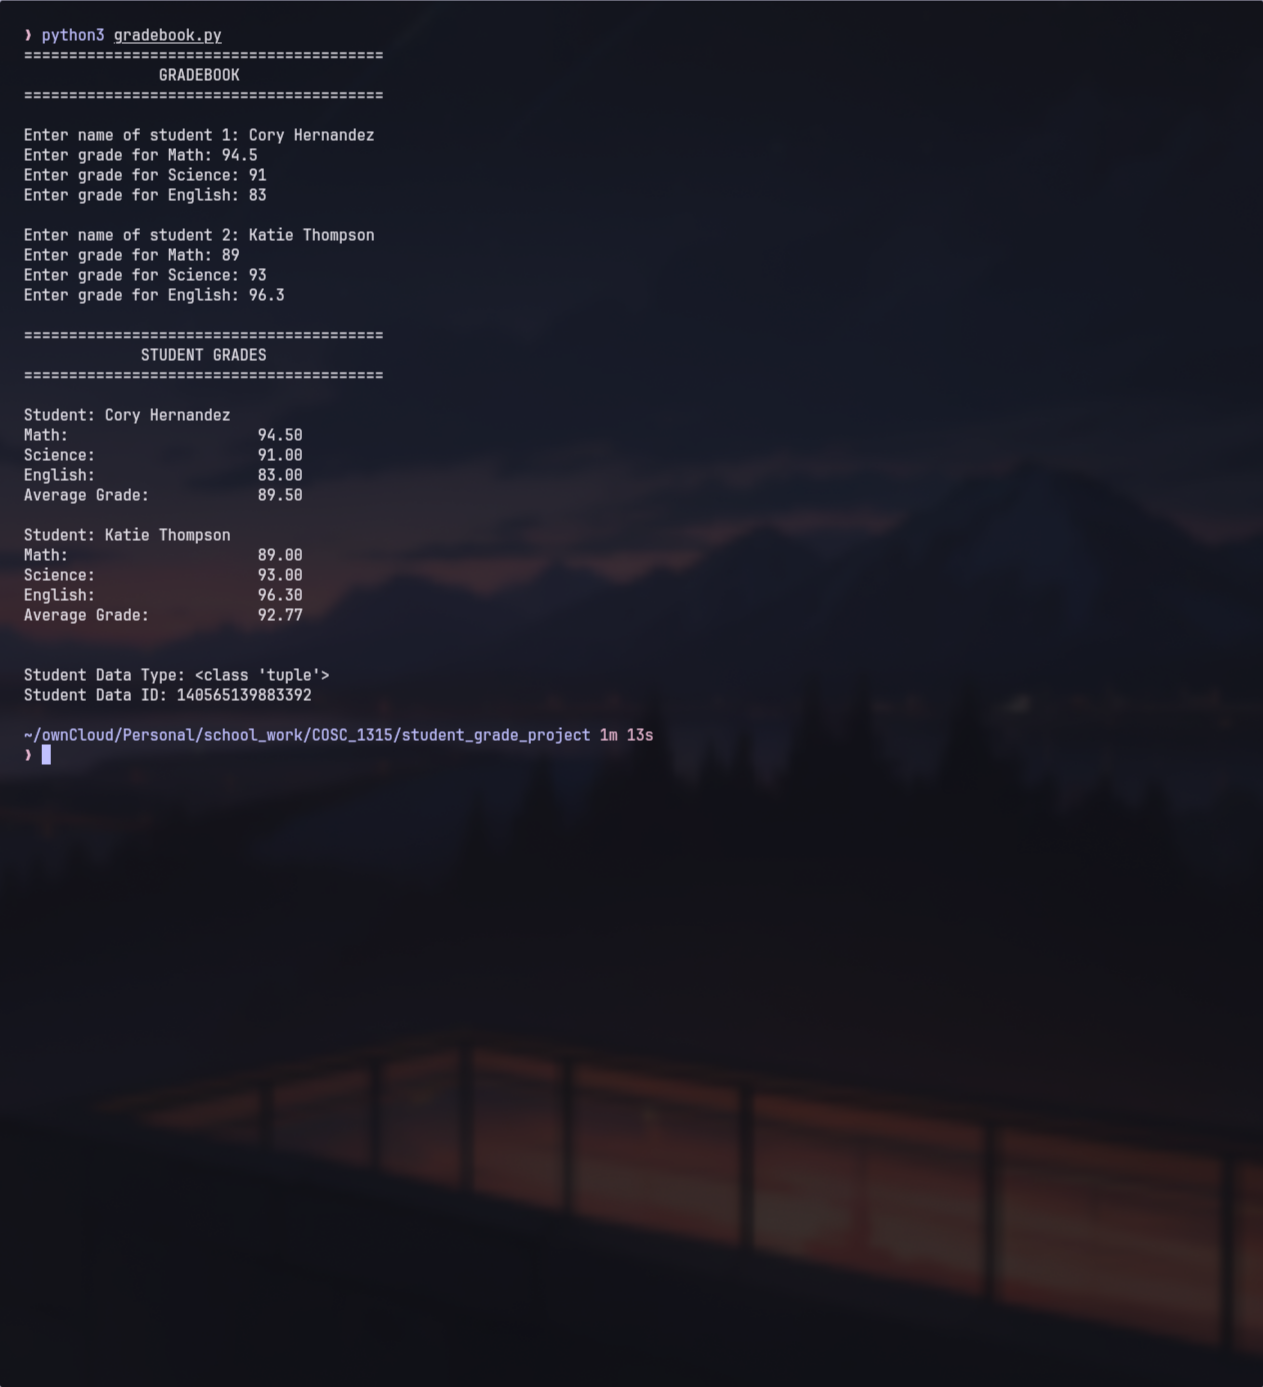
\includegraphics[width=1\textwidth]{gradebook_function.png}
    \caption{Output of gradebook program.}
    \label{fig:functionality}
  \end{figure}

\begin{figure}[H]
    \centering
    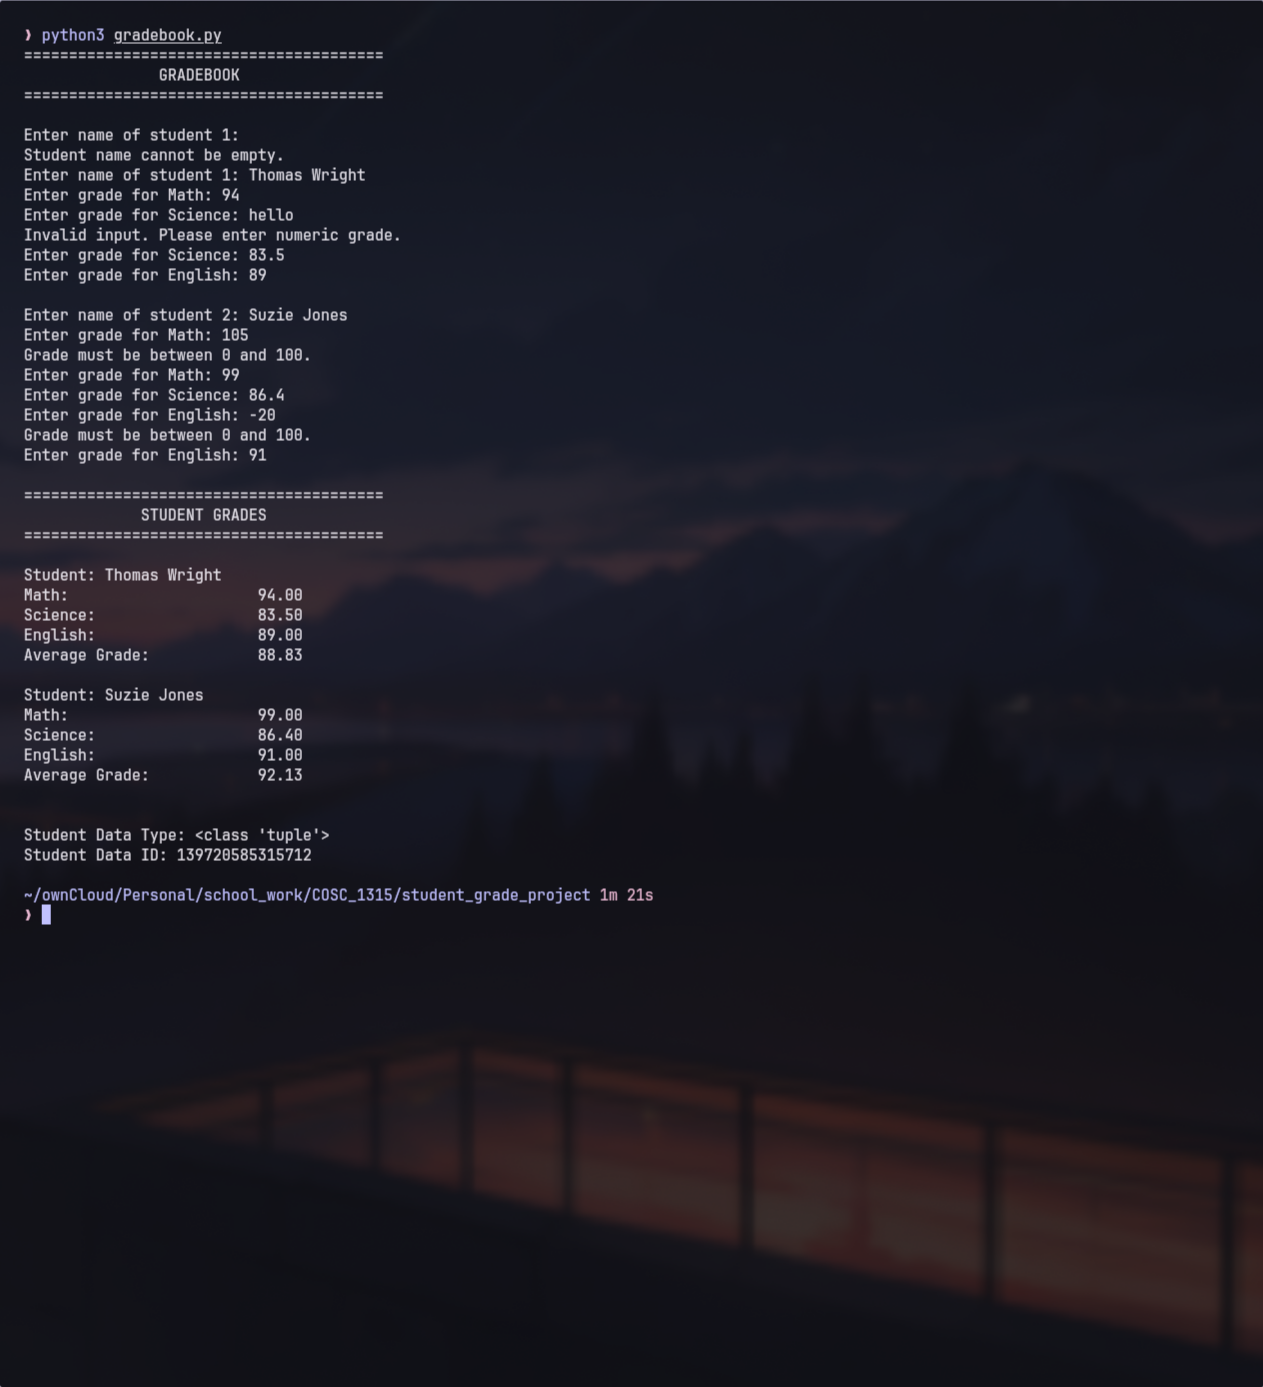
\includegraphics[width=1\textwidth]{gradebook_function_errors.png}
    \caption{Output of gradebook program showing error handling.}
    \label{fig:functionality}
  \end{figure}


\end{document}
